\documentclass[danish]{article}

\usepackage{fullpage} 
\usepackage[latin1]{inputenc} 
\usepackage[danish]{babel}
\usepackage{listings} 
\usepackage{caption}
\usepackage{subcaption}
\usepackage{xcolor}
\usepackage{amssymb} 
\usepackage{amsmath} 
\usepackage{fancyhdr}
\usepackage{lastpage} 
\usepackage{hyperref}
\usepackage{parskip} 
\usepackage{graphicx} 
\usepackage{pdfpages}
\usepackage{abstract}
\usepackage{url}
\usepackage{float}

% setup c sharp syntax highlight 
\lstdefinestyle{sharpc}{ language=[Sharp]C,
frame=lr, rulecolor=\color{black}, basicstyle=\footnotesize\ttfamily,
keywordstyle=\bfseries\color{green!40!black},
commentstyle=\itshape\color{purple!40!black}, identifierstyle=\color{blue},
stringstyle=\color{orange}}

\lstset{ style=sharpc, numbers=left, escapeinside={\<*}{*>},
breakatwhitespace=true }

% code formatting helper 
\newcommand{\code}[1]{\texttt{#1}}

% no paragraph indention 
\setlength{\parindent}{0pt}

% setup page style 
\pagestyle{fancy} 
\fancyhf{} 
\setlength{\headheight}{15pt}
\setlength{\headsep}{25pt} 
\lfoot{Side \thepage{} af \pageref{LastPage}}
\rfoot{13/05-2013} \lhead{02161 Software Engineering 1} 
\chead{Obligatorisk opgave} 
\rhead{Gruppe 17}

\author{
  Patrick Gadd\\
  \texttt{s113491}
  \and
  Markus F�revaag\\
  \texttt{s123692}
  \and
  Simon Altschuler\\
  \texttt{s123563}
}
\title{02161 Software Engineering\\
  Obligatorisk opgave}
\date{13/05-2013}

\begin{document}
\maketitle
\bf{Gruppe 17}
\clearpage

\section{Introduction} 
In this assignment we have attempted to meet the requirements of the assignment, but have gone a step further by adding a persistency layer as well as a graphical user interface. We realize that these were not part of the essential assignment, but while in the initial planning and designing phase, we agreed on finding it would be easier to implement the system that way from the beginning. That is true for both the persistency and the GUI alike.

Section \ref{requirements} describes our perception of the customers wishes through a glossary and six use cases. This part is very important in real life, as it is used to align expectations between the costumer and developer.

Section \ref{architecture} is a description of the design of the application through class diagrams as well as three sequence diagrams. This part has it's real-life use amongst the actual developers working on an application, as it makes the code more manageable to the developers - especially newcomers.

\section{Requirements Specification}
\label{requirements}
\subsection{Important concepts}
\begin{description}
\item[Project] \hfill \\
A project is basically a collection of activities. Is has an assigned managing user, a name and a budget limit.  

\item[Activity] \hfill \\
The activity is what constitues actual work tasks in a project. They each have their own budget and description. Developers can be assigned to work on activities, and they register time by choosing which activity that entry belongs to.

\item[Fixed activity] \hfill \\
A fixed activity is just an activity, but it is not linked to a specific project. Instead it is a way for users to register time that has no project reference, but instead is either due to sickness, vacation, courses, etc.

\item[Developer] \hfill \\
All users in the system are also (or can be) developers. They are the ones who register time, create users and projects and generally maintain the system. Nothing can be accessed without a valid login. They have a name and their initials stored.

\item[Project Manager] \hfill \\
The project manager is just a user, who is assigned as a manager on a project. They are the ones who are responsible for activities in a project and assigns developers to work on specific activites.

\item[Assistance] \hfill \\
A developer may ask another developer to help out on an activity. The assisting user then registers the used time normally, except he now flags the entry as an assist. A user does not need to be assigned to an activity to assist on it.

\item[Budgets] \hfill \\
All budgets in the system are represented by a number of hours that a project or activity is estimated to last. There is both project budgets and activity budgets so that the project managers can easily see how much of a project budget is currently estimated to be used by current activities.

\item[Report] \hfill \\
The project report is a screen in which the project managers can view statistics about the project. There are figures and numbers describing how much of the budget is in use and how much time is estimated to be left, and how much time has been registered to that project in total.

\end{description}

\subsection{Use cases}
\begin{table}[H]
  \begin{tabular}{|l|l|}
    \multicolumn{2}{l}{
      \bf{Create a new project}
    }
    \\ \hline
    Description & A developer creates a new project 
    \\ \hline
    Actor & User
    \\ \hline \multicolumn{2}{|l|}{
      Main scenario 
    }
    \\ \hline \multicolumn{2}{|l|}{ \parbox{\textwidth}{
        \begin{enumerate}
        \item{The user logs in (if not already logged in)}
        \item{The user clicks the ``Projects'' button in the top bar menu}
        \item{The user fills out the ``Name'', ``Deadline'' and ``Budgetted hours'' fields}
        \item{The user decides whether or not to assign a manager}
          \begin{itemize}
          \item {If yes, the user selects the user from the ``Manager'' drop down list}
          \end{itemize}
        \item{The user clicks the ``Create new'' button}
        \item{The new project is displayed in above the list of all projects}
        \end{enumerate}
      }}
    \\ \hline \multicolumn{2}{|l|} {
      Alternative scenarios }
    \\ \hline \multicolumn{2}{|c|}{\parbox{\textwidth}{
        \begin{enumerate}
        \item{The user does not fill in one or more of the three mandatory fields (``Name'', ``Deadline'' and/or ``Budgetted hours'')}
          \begin{itemize}
          \item {The user is prompted to fill in all fields, and no project is created}
          \end{itemize}
        \item{The user inputs an invalid date}
          \begin{itemize}
          \item{The user is prompted to format the date correctly, and no project is created}
          \end{itemize}
        \item{The user inputs an invalid number of hours}
          \begin{itemize}
          \item{The user is prompted to input a valid number of hours, and no project is created}
          \end{itemize}
        \end{enumerate}
      }}
    \\ \hline
  \end{tabular}
\end{table}

\begin{table}[h]
  \begin{tabular}{|l|l|}
    \multicolumn{2}{l}{
      \bf{Remove a developer}
    }
    \\ \hline
    Description & A developer is fired or quits, and his/hers user must be removed
    \\ \hline
    Actor & User
    \\ \hline \multicolumn{2}{|l|}{
      Main scenario 
    }
    \\ \hline \multicolumn{2}{|l|}{ \parbox{\textwidth}{
        \begin{enumerate}
        \item{The user logs in (if not already logged in)}
        \item{The user clicks the ``Developers'' button in the top bar menu}
        \item{The user selects the developer that must be deleted}
        \item{The user clicks the ``Delete selected'' button}
        \item{The user accepts a prompt to confirm the deletion}
        \item{The developer is removed from the above list of developers}
        \item{The deleted developer's registered time entries, activity- and manager assignments are all deleted from the system}
        \end{enumerate}
      }}
    \\ \hline \multicolumn{2}{|l|} {
      Alternative scenarios }
    \\ \hline \multicolumn{2}{|c|}{\parbox{\textwidth}{
        \begin{enumerate}
        \item{The user tries to remove his/hers own account}
          \begin{itemize}
          \item {The user is prompted and told it cannot be done}
          \end{itemize}

        \item{The user denies the prompt to delete the develper}
          \begin{itemize}
          \item {The user is taken to the initial ``Developers'' screen, and no developer is deleted}
          \end{itemize}

        \item{The user clicks ``Delete selected'' button while no developer is selected}
          \begin{itemize}
          \item {The user is told that no developer is selected, and no developer is deleted}
          \end{itemize}
        \end{enumerate}
      }}
    \\ \hline
  \end{tabular}
\end{table}

\begin{table}[H]
  \begin{tabular}{|l|l|}
    \multicolumn{2}{l}{
      \bf{Generate report}
    }
    \\ \hline
    Description & A developer wants to see a report on a project
    \\ \hline
    Actor & User (a developer)
    \\ \hline \multicolumn{2}{|l|}{
      Main scenario 
    }
    \\ \hline \multicolumn{2}{|l|}{ \parbox{\textwidth}{
        \begin{enumerate}        
        \item{At their weekly project-meetings, developers must be able to see how the projects are progressing}
        \item{On each project it should be possible to see information about}
          \begin{description}
          \item[The total number of activities on the project] {}

          \item[Progress on each activity?! Har vi ikke implementeret TODO] \hfill \\
            {Should be calculated the following way...}

          \item[How much of the budgeted time has been allocated to activities]\hfill \\
            {Should be calculated the following way:
              The sum of budgeted hours on all of the project's activities}

          \item[How much work has been registered]\hfill \\
            {Should be calculated the following way:
              The sum of registered hours on all of the project's activities
              Kommer assists med? TODO}

          \item[An estimate on percentage completion]\hfill \\
            {TODO Should be calculated the following way:}

          \item[An estimate on overall remaining man-hours]\hfill \\
            {Should be calculated the following way:}
          \end{description}
        \end{enumerate}
      }}
    \\ \hline \multicolumn{2}{|l|} {
      Alternative scenarios }
    \\ \hline \multicolumn{2}{|c|}{\parbox{\textwidth}{
        \begin{enumerate}
        \item{Budget is exceeded by sum of hours registered compared to project budget}
          \begin{itemize}
          \item {Mark in red color}
          \end{itemize}
        \item{Budget is exceeded by accumulated sum of bugdgetted hours of activites on project }
          \begin{itemize}
          \item{Mark in red color}
          \end{itemize}
        \end{enumerate}
      }}
    \\ \hline
  \end{tabular}
\end{table}

\begin{table}[H]
  \begin{tabular}{|l|l|}
    \multicolumn{2}{l}{
      \bf{Add a developer}
    }
    \\ \hline
    Description & A developer is hired and must be added to the system 
    \\ \hline
    Actor & User (another developer)
    \\ \hline \multicolumn{2}{|l|}{
      Main scenario 
    }
    \\ \hline \multicolumn{2}{|l|}{ \parbox{\textwidth}{
        \begin{enumerate}
        \item{A developer is hired and needs a login}
        \item{The user fills in initials and full name of the new developer, and creates the new account}
        \end{enumerate}
      }}
    \\ \hline \multicolumn{2}{|l|} {
      Alternative scenarios }
    \\ \hline \multicolumn{2}{|c|}{\parbox{\textwidth}{
        \begin{enumerate}
        \item{The user forgets to fill in a name}
          \begin{itemize}
          \item {The user should be prompted, and no new account should be created}
          \end{itemize}
		  
		  \item{The user forgets to fill in initials}
          \begin{itemize}
          \item {The user should be prompted, and no new account should be created}
          \end{itemize}

        \item{The length of the initials is greater than 4}
          \begin{itemize}
          \item {The user should be prompted, and no new account should be created}
          \end{itemize}
        \end{enumerate}
      }}
    \\ \hline
  \end{tabular}
\end{table}
\begin{table}[H]
  \begin{tabular}{|l|l|}
    \multicolumn{2}{l}{
      \bf{Register time entry - By Markus Færevaag}
    }
    \\ \hline
    Description & A developer has spent time on an activity and needs to register that time in the system
    \\ \hline
    Actor & User
    \\ \hline \multicolumn{2}{|l|}{
      Main scenario 
    }
    \\ \hline \multicolumn{2}{|l|}{ \parbox{\textwidth}{
        \begin{enumerate}
        \item{The developer logs in (if not already logged in)}
        \item{The user clicks the ``Register time'' button on the top menu bar}
        \item{The user then types in what date and time span have been spent on the activity}
        \item{The user chooses if the activity should be fixed}
          \begin{itemize}
          \item {If yes, the user then chooses which kind of fixed activity (eg. vacation, sickness, course etc)}
            \item{If no, the user chooses the project and in turn the activity which has been worked on. Only projects and activities that the developer is assigned to is displayed}
          \end{itemize}
        \item{The user presses the ``Register'' button to register the time}
        \item{The time entry is now displayed in the above calendar view as an orange colored slot which size represents the time span}
        \end{enumerate}
      }}
    \\ \hline \multicolumn{2}{|l|} {
      Alternative scenarios }
    \\ \hline \multicolumn{2}{|c|}{\parbox{\textwidth}{
        \begin{enumerate}
        \item{The user has marked non-fixed activity and has not selected a project and/or activity}
          \begin{itemize}
          \item {The user is told that a project and activity must be selected, and no time entry will be registered}
          \end{itemize}

        \item{The user inputs an invalid date}
          \begin{itemize}
          \item {The user is told that the date is invalid, and no time entry will be registered}
          \end{itemize}

        \item{The user inputs an invalid time in either start or end time}
          \begin{itemize}
          \item {The user is told that the time is invalid, and no time entry will be registered}
          \end{itemize}

        \item{The user tries to register time which overlaps existing time entries}
          \begin{itemize}
          \item {The user is told that the time entry overlaps existing entries, and no time entry will be registered}
          \end{itemize}

        \end{enumerate}
      }}
    \\ \hline
  \end{tabular}
\end{table}
\begin{table}[H]
  \begin{tabular}{|l|l|}
    \multicolumn{2}{l}{
      \bf{Create a new activity}
    }
    \\ \hline
    Description & A new activity needs to be added to a project
    \\ \hline
    Actor & User
    \\ \hline \multicolumn{2}{|l|}{
      Main scenario 
    }
    \\ \hline \multicolumn{2}{|l|}{ \parbox{\textwidth}{
        \begin{enumerate}
        \item{The user logs in (if not already logged in)}
        \item{The user clicks ``Projects'' button in the top bar menu}
        \item{The user selects the project to which the activity should be added}
        \item{The user clicks the ``Maintain selected'' button}
        \item{The user fills out ``Name'', ``Hour budget'' and ``Deadline'' fields}
        \item{The user clicks the ``Add activity'' button}
        \item{The new activity is displayed in the above list of all activities in the current project}
        \end{enumerate}
      }}
    \\ \hline \multicolumn{2}{|l|} {
      Alternative scenarios }
    \\ \hline \multicolumn{2}{|c|}{\parbox{\textwidth}{
        \begin{enumerate}
        \item{The user inputs an invalid date}
          \begin{itemize}
          \item {The user is told to use a valid date, and no activity is created}
          \end{itemize}

        \item{The user inputs an invalid number in the ``Hour budget'' field}
          \begin{itemize}
          \item {The user is told to type in a valid number, and no activity is created}
          \end{itemize}

        \item{The user does not fill out all fields}
          \begin{itemize}
          \item {The user is told to fill out all fields, and no activity is created}
          \end{itemize}
        \end{enumerate}
      }}
    \\ \hline
  \end{tabular}
\end{table}


\subsection{Limiting}
We have not made very many compromises regarding the functionalities described in the specifications. We decided from the beginning to implement a GUI, but also knew that we would not be spending much time styling and visually designing it. This is somewhat reflected in the final result, even though we find it good enough to actually be useable.

We were a little confused about some of the features described. For instance, at first we thought the sentence ``Projektlederen skal gradvis opdele projektet i aktiviteter'' meant that activities should be dividable after their creation. Later on we agreed that this was not the case and dropped development of that particular feature. Also we were not excatly sure what the project report had to show or do, so we thought up a solution that met the requirements as we understood them, and seemed useful.


\section{Program Architecture}
\label{architecture}
\subsection{Class Diagrams}
\begin{figure}[H]
  \centering
  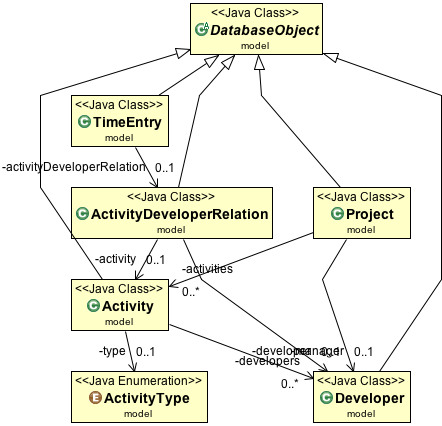
\includegraphics[width=10cm]{uml/model-simple-uml.png}
  \label{fig:model_uml}
  \caption{The model architecture.}
\end{figure}

\begin{figure}[H]
  \centering
  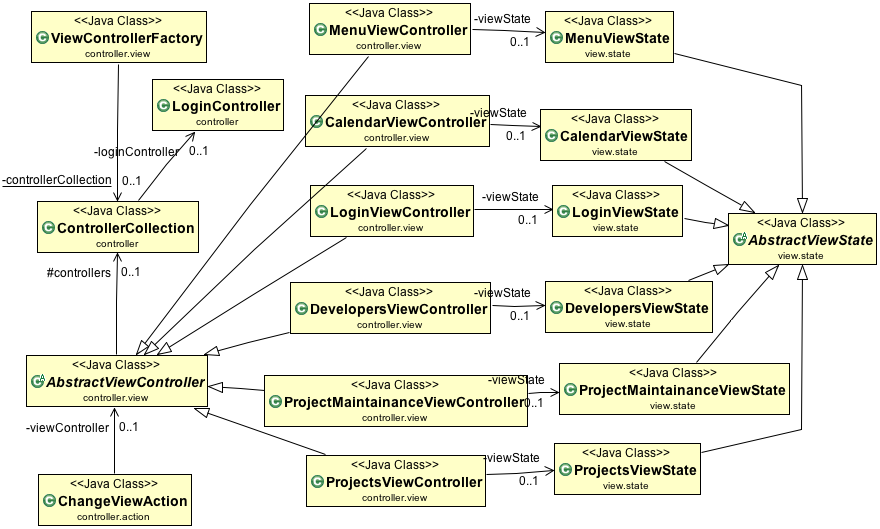
\includegraphics[width=15cm]{uml/controller-simple-uml.png}
  \label{fig:vc_uml}
  \caption{The view-controller architecture.}
\end{figure}


\begin{figure}[H]
  \centering
  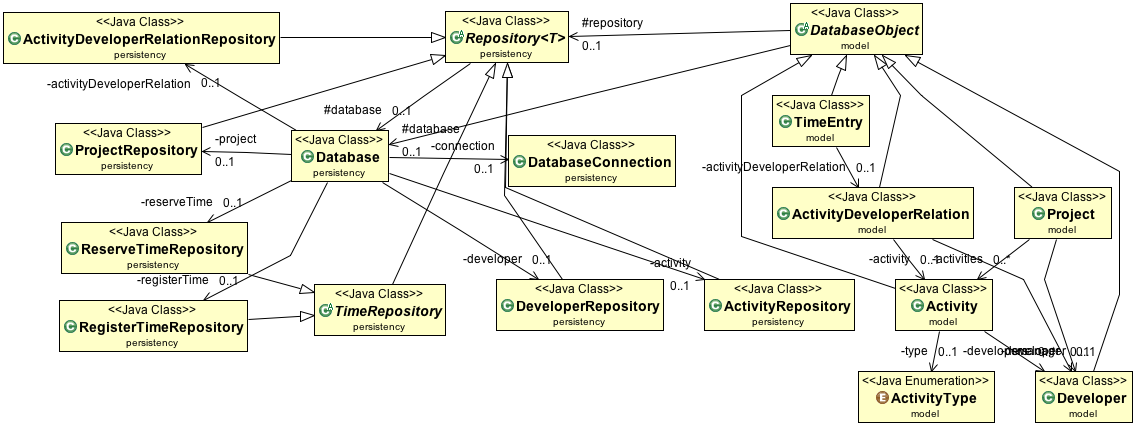
\includegraphics[width=15cm]{uml/model-persistency-simple-uml.png}
  \label{fig:persistency_uml}
  \caption{The persistency architecture.}
\end{figure}

\subsection{Sequence Diagrams}
Please see the attached file named \code{sequence.zip} for the three sequence diagrams. 

\subsection{Architecture Design}
We are using SQLite as our database. We use ``SQLite JDBC Driver''\footnote{\url{https://bitbucket.org/xerial/sqlite-jdbc}} as the driver, which allows us to execute arbitrary SQL commands very conveniently. On top of this driver lies our persistency module, which exposes an API to work with the different data models, by abstracting away actual SQL command calls.

For each table in the database, there is a corresponding Java class, which maps each column to a property. This is shown in figure 1. These are all based on a very simple class, \code{DatabaseObject}, which has a single property, the \code{id}. This is used to identify the entity in the database, and is the only trusted identifier for an object. 

There is a repository for each model object, which exposes a \code{CRUD} interface for working with that model. Repositories have access to each other, so that they can fetch data about their own attributes easily. For instance, an \code{Activity} can fill out its \code{project} property, by asking the \code{ProjectRepository} for a \code{Project} model.

We created a class, \code{Query}, that somewhat resembles \code{C\#}s \code{LINQ}\footnote{\url{http://msdn.microsoft.com/en-us/library/vstudio/bb397926.aspx}}. It allows us to completely abstract the string based SQL statements away by building \code{Query} objects and chain methods (by return its own instance). This greatly reduces the risk of simple typos and the like.

The repositories are used by \code{ViewControllers}, which are (as the name implies), control the \code{View}s. They contain the business logic code, as they fetch data from the repositories, and send it to the \code{View}s, who then displays them accordingly. This is illustrated in figure 3.

The \code{View}s are completely isolated objects, who know nothing of the other parts of the application, and other parts of the application know nothing of how they display the data. This is reflected in figure 2, where they are the last part of the dependency chain.

This means that the actual GUI could easily be interchanged with a CLI\footnote{Command Line Interface}, or some other interface, except for the fact that there are some \code{Swing} components that the \code{ViewController}s make use of (for instance, adding a handler to a button). This could have been avoided by using Interfaces, but we felt that it was beyond the scope of this project.

\section{Testing}
This is a test
\subsection{Add developer}
\subsection{Use case: Add Developer}


Input partitions
\begin{center}
  \begin{tabular}{| l | l |}
    \hline
	Input data set & Input property \\ \hline
    1 & Initials and name \\ \hline
    2 & Name only \\ \hline
    3 & Initials only \\ \hline
	4 & Name and too many initials \\
    \hline
  \end{tabular}
\end{center}


Test values \& expected output
\begin{center}
  \begin{tabular}{| l | l | l |}
    \hline
	Input data set & Contents & Expected output \\ \hline
    1 & ``MD'' \& ``Moby Dick'' & the total developer count is increased by 1 \\ \hline
	2 & ``'' \& ``Moby Dick'' & \begin{tabular}[x]{@{}l@{}}the total developer count is not affected, \\and the user is prompted\end{tabular} \\ \hline
    3 & ``MD'' \& ``'' & \begin{tabular}[x]{@{}l@{}}the total developer count is not affected, \\and the user is prompted\end{tabular} \\ \hline
    4 & ``12345'' \& ``Moby Dick'' & \begin{tabular}[x]{@{}l@{}}the total developer count is not affected, \\and the user is prompted\end{tabular} \\
    \hline
  \end{tabular}
\end{center}
\subsection{Create new activity}
\subsection{Use case: Create a new activity}

Input partitions
\begin{center}
  \begin{tabular}{| l | l |}
    \hline
	Input data set & Input property \\ \hline
    1 & Description, hour budget and deadline \\ \hline
    2 & Hour budget and deadline only \\ \hline
    3 & Description and deadline only \\ \hline
    4 & Description and hour budget only \\ \hline
    5 & Description, negative hour budget and deadline  \\ \hline
    6 & Description, hour budget and deadline which has already passed \\ \hline
    7 & Description, hour budget and malformed deadline dates \\ \hline
  \end{tabular}
\end{center}

Test values \& expected output

Input partitions
\begin{center}
  \begin{tabular}{| l | l | l |}
    \hline
	Input data set & Contents & Expected output \\ \hline
    1 & "Swim with Moby Dick", \\ & "123", "22-04-2666" & Activity created \\ \hline
    2 & "\ ", "123", "22-04-2666" & "You must fill out all fields!" \\ \hline
    3 & "Swim with Moby Dick", \\ & "\ ", "22-04-2666" & "You must fill out all fields!" \\ \hline
    4 & "Swim with Moby Dick", \\ & "123", "\ " & "You must fill out all fields!" \\ \hline
    5 & "Swim with Moby Dick", \\ & "-1", "22-04-2666" & "Hour budget cannot be negative!" \\ \hline
    6 & "Swim with Moby Dick", \\ & "123", "01-01-1991" & "You can't make a deadline which \\ && is already passed" \\ \hline
    7 & "Swim with Moby Dick", \\ & "123", "asdf" & "Invalid date format, you must \\ & & use dd-mm-yyyy" \\ \hline
  \end{tabular}
\end{center}


\section{Conclusion}
This is a conclusion

\section{Appendix}
\subsection{Original schedule document}
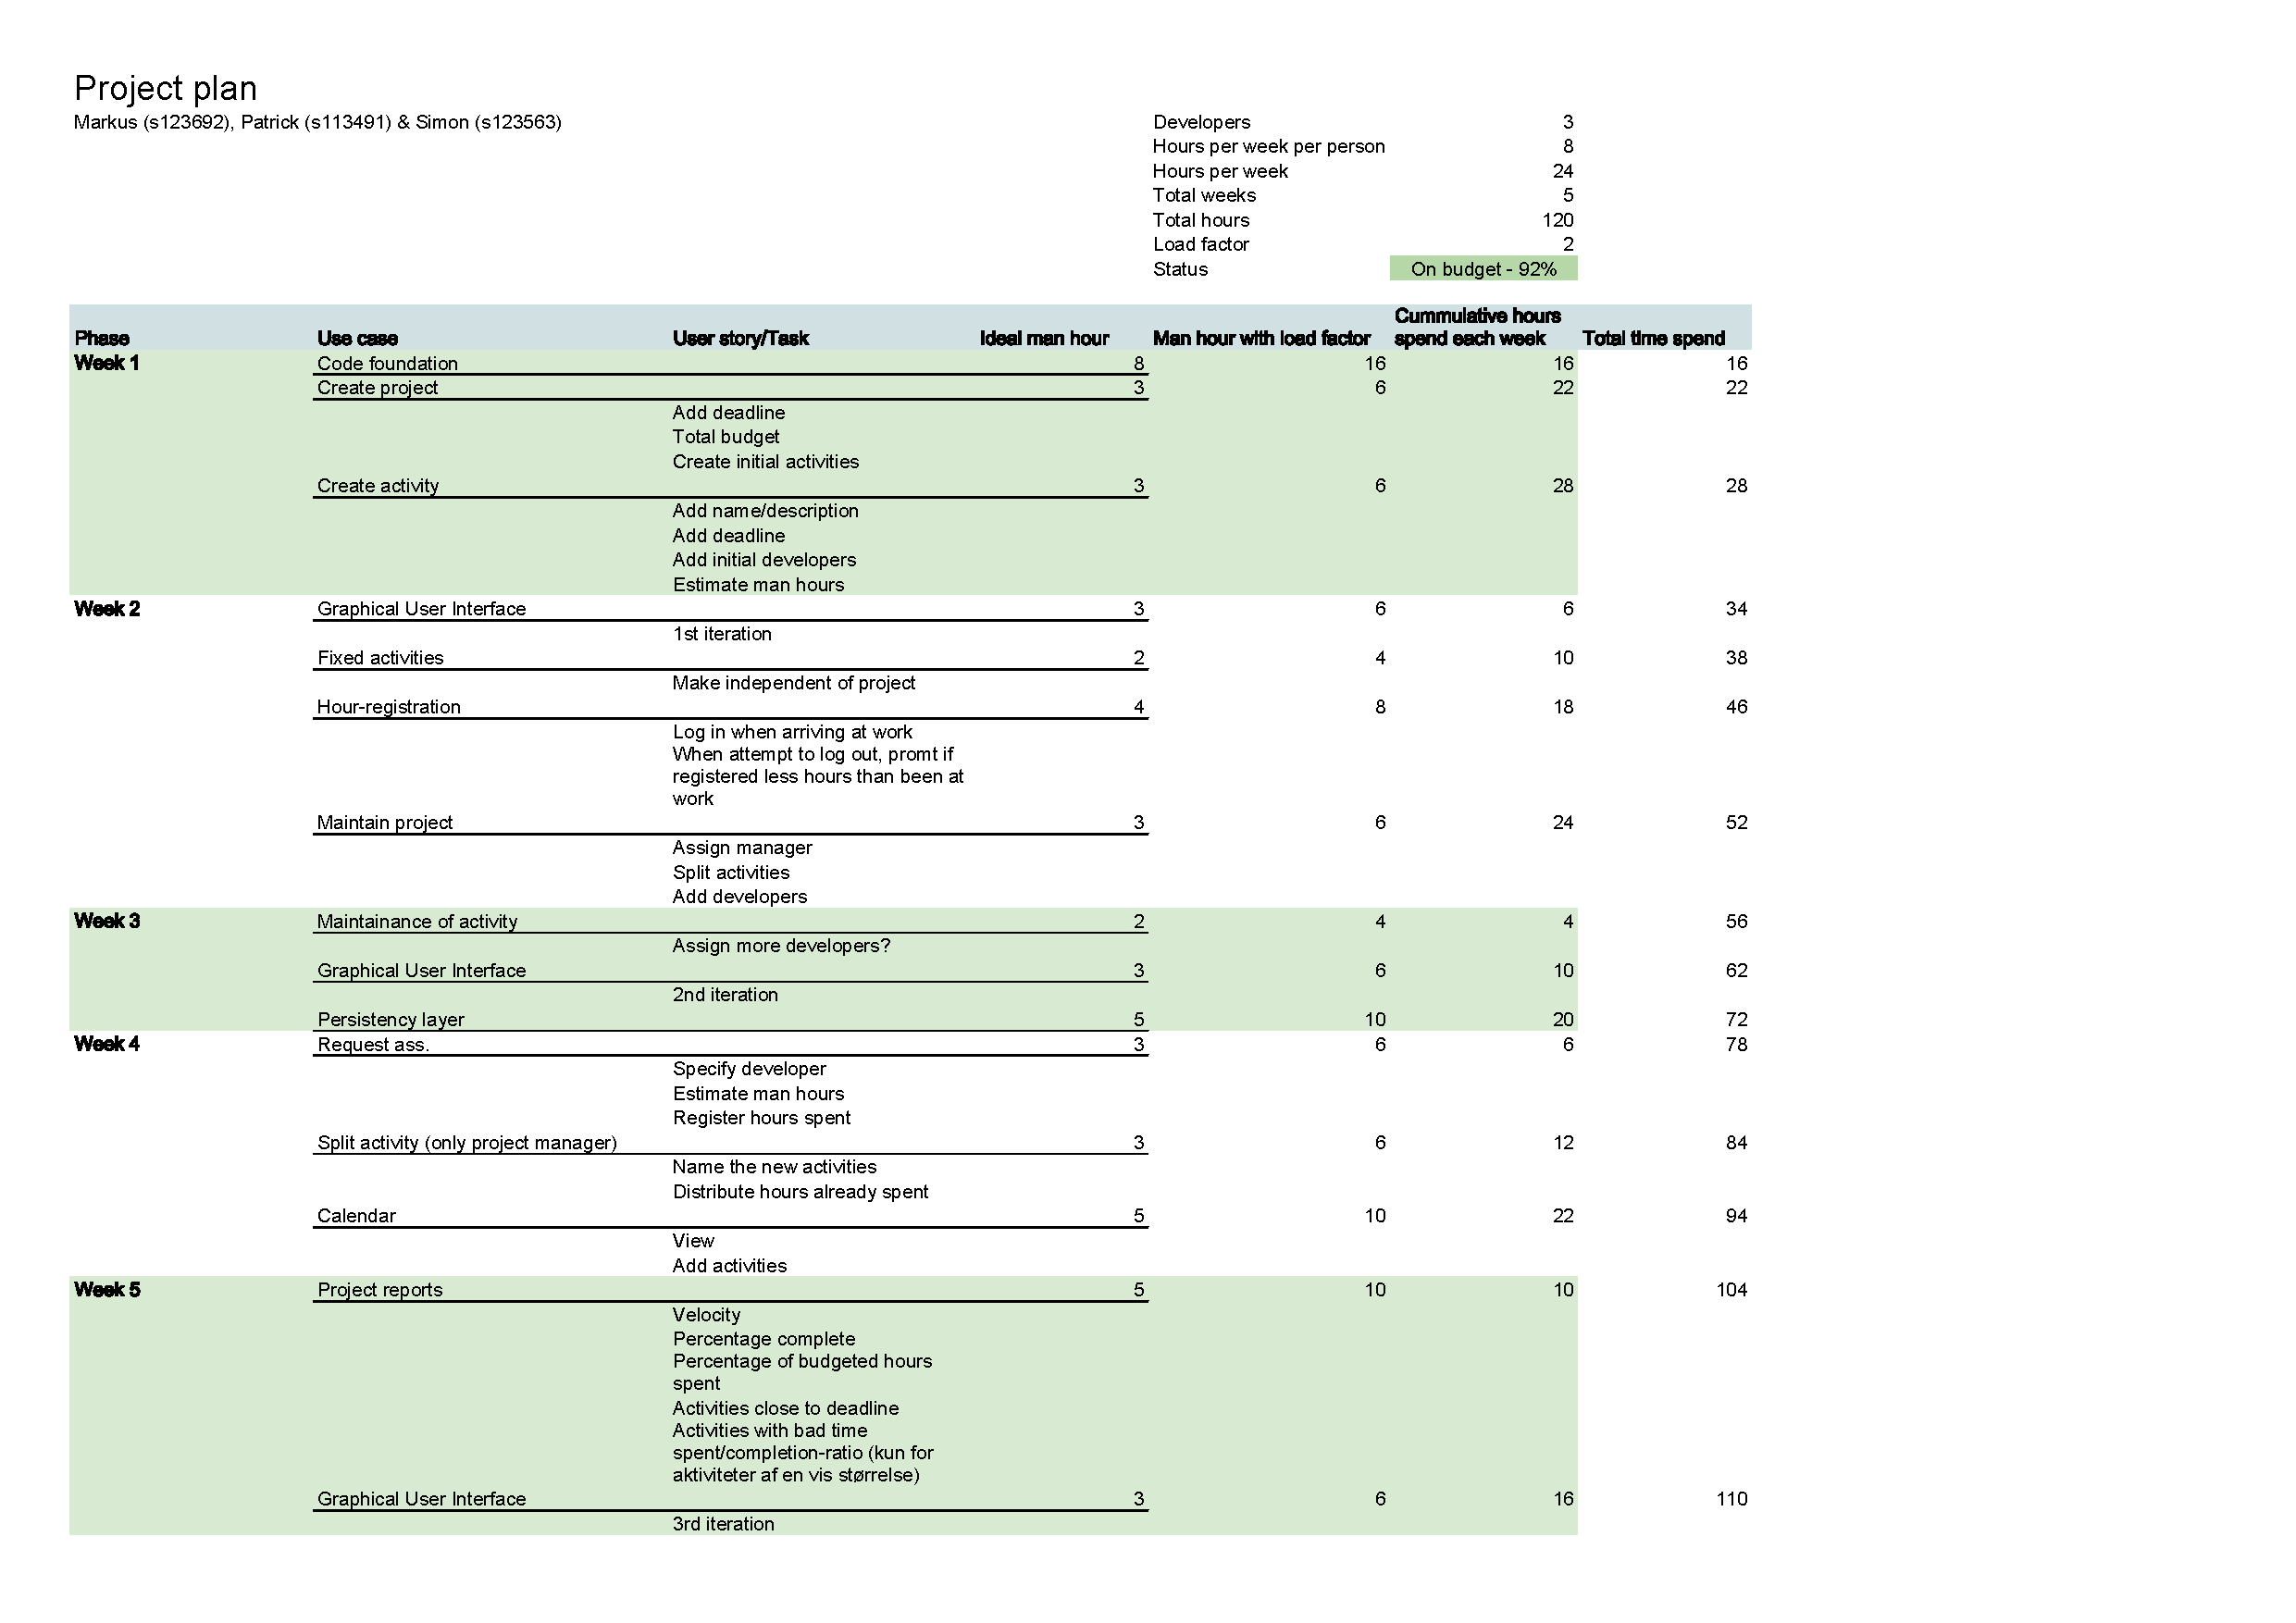
\includepdf{projekt_plan_gruppe_17.pdf}

\end{document}